\subsection{Appearance editor}
\writer{Monica}

The Appearance Editor is the component which allows the user to associate a visual representation to the Petri net elements so that they can be represented in the 3D simulation. The editor can be used by both technical and non-technical users as it only implies linking \textit{Appearance Labels} previously defined in the Petri net with predefined 3D or texture files. 

Figure \ref{fig:appearance} shows the model used by the Appearance Editor component.

\begin{figure}[htp]
\begin{center}
  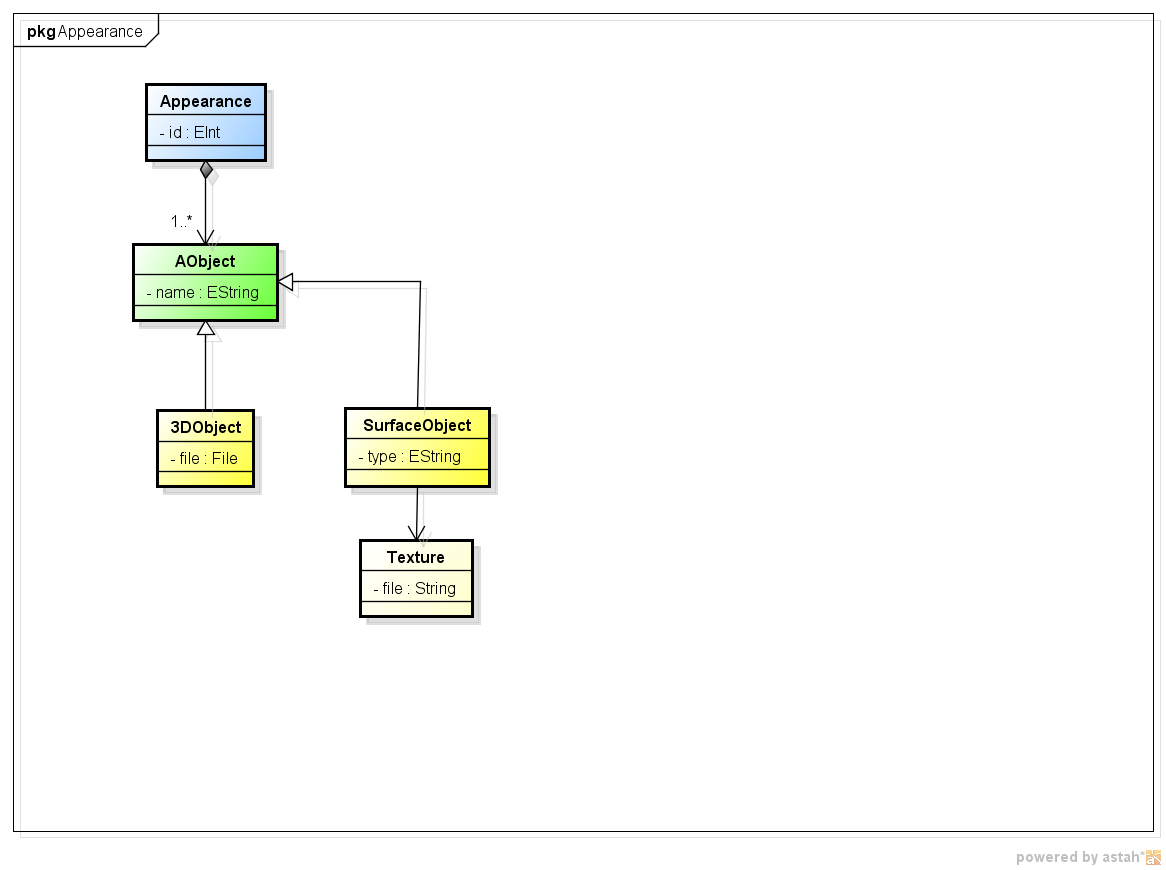
\includegraphics[width=0.8\textwidth]{image/appearance-model.png}
  \caption{Appearance Domain Model}
  \label{fig:appearance}
\end{center}
\end{figure}  

\subsubsection{Appearance Editor classes}
Next, the model will be described into more detail.

\paragraph{Appearance}
The Appearance class is simply an abstract definition of an Appearance object.

\paragraph{AObject}
The AObject class is general class from which different appearance objects will inherit. Its only attribute, \textbf{name}, refers to the name of the object that is represented by this appearance (e.g. \textit{"train"}).

\paragraph{3DObject}
The 3DObject class consists of only one attribute,\textbf{file}, of type String, which represents the path of the 3D model on the hard disk. Also, 3DObject will inherit from AObject.

\paragraph{SurfaceObject}
The SurfaceObject class consists of only one attribute, \textbf{type}, of type String, which represents the shape of the object to be visualized (e.g. \textit{"rectangular"}). SurfaceObject will also inherit from AObject.

\paragraph{Texture}
The Texture class consists of only one attribute,\textbf{file}, of type String, which represents the path of the texture model on the hard disk.


